\section{Durchführung}
\label{sec:Durchführung}

Der grundlegende Aufbau des Versuchs ist in Abbildung \ref{fig:aufbau} dargestellt.

\begin{figure}[H]
  \centering
  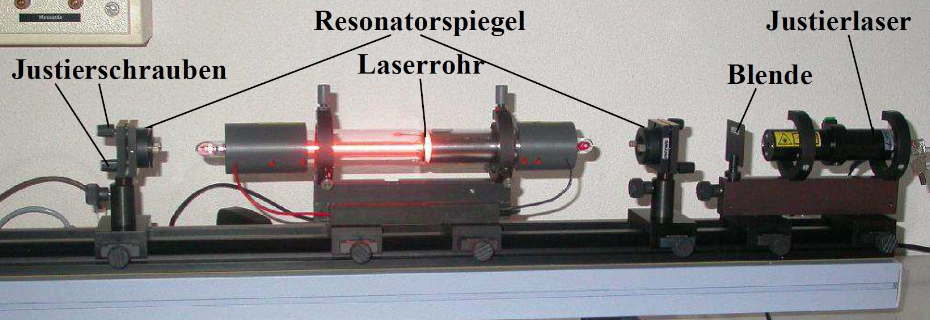
\includegraphics[height=5cm]{Aufbau.PNG}
  \caption{Der Grundlegende Aufbau des Versuchs. \cite{sample}}
  \label{fig:aufbau}
\end{figure}

Auf einer optischen Schiene befinden sich ein Laserrohr und zwei Resonatorspiegel
sowie ein Justierlaser mit einer davor befindlichen Blende.

Zu Beginn muss die gesamte Apparatur justiert werden. Dazu wird der Justierlaser
eingeschaltet und es werden nacheinander die beiden Resonatorspiegel vor diesen
gestellt. Dabei werden jeweils die Justierschrauben der Spiegel so eingestellt,
dass der reflektierte Laserstrahl wieder möglichst mittig auf die Blende vor dem
Justierlaser zurückgeworfen wird. Anschließend werden die Spiegel entsprechend
der Abbildung in gleichem Abstand neben dem eigentlichen Laserrohr platziert. Nun kann nach einer
erneuten Feinjustage der Schrauben der Laserbetrieb aufgenommen werden. Der Justierlaser
wird abgeschaltet.

Im ersten Versuchsteil wird dann die Stabilitätsbedingung der Laserapparatur überprüft.
Dazu wird mit einer Diode, die hinter dem zweiten Resonatorspiegel auf der optischen
Bank angebracht wird, die Intensität des Laserstrahls in Abhängigkeit des Abstandes
der beiden Spiegel zueinander gemessen. Dies wird für zwei Resonatorkonfigurationen
durchgeführt. Bei der ersten wird ein planarer und ein konkaver (Krümmungsradius $\SI{1400}{\milli\meter}$)
Spiegel verwendet. Die zweite Konfiguration besteht aus zwei konkaven Spiegeln
(Krümmungsradius jeweils $\SI{1400}{\milli\meter}$). Nach Vergrößerung des Abstandes
werden die Schrauben der Resonatorspiegel in jedem Schritt nachjustiert.

Im zweiten Versuchsteil wird dann bei festem Abstand der Resonatorspiegel eine
Streulinse vor der Diode platziert. Dadurch entsteht an der Diode eine Abbildung
der Grundmode. Die Diode ist horizontal beweglich auf einer
Schiene angebracht. So wird mit ihrer Hilfe der Intensitätsverlauf des gestreuten
Laserstrahls (also der Grundmode) in der Ebene senkrecht zur Strahlrichtung gemessen.
Die gleiche Messung wird noch einmal wiederholt, jedoch wird nun zusätzlich ein
Draht zwischen Laserrohr und hinterem Resonatorspiegel platziert, sodass sich nun
eine Abbildung der ersten Mode an der Diode ergibt.

Anschließend soll dann die Polaritation des Laserstrahls untersucht werden. Dazu
wird der Draht wieder entfernt und die Streulinse wird durch einen Polarisationsfilter
ersetzt. Sodann wird mit der Diode die Intensität des Strahls bei unterschiedlichen
Stellungen des Polarisationsfilters gemessen.

Im letzten Versuchsteil wird der Filter dann noch durch ein Gitter ersetzt, wodurch
sich auf einem am Ende des Versuchsaufbaus befindlichen Schirm ein entsprechendens
Interferenzmuster ergibt. Es wird der Abstand des Gitters zum Schirm und die Abstände
der Maxima erster Beugungsordnung zum Maximum nullter Ordnung bestimmt.
